% document type (MUST HAVE)
\documentclass[letterpaper, 12pt]{article}

% 1 inch margin
\usepackage[margin=1in]{geometry}

% 24pt paragraph indentation
% there is auto indentation at every new paragraph which is separated by a blank line
% paragraph 1
%
% paragraph 2
\setlength\parindent{0pt}

% font (fontspec can only be used with lualatex or xetex compiler engine)
% default compiler engine is pdftex
\usepackage{fontspec}
\setmainfont{Calibri}

% images
\usepackage{graphicx}
\graphicspath{ {../screenshots/} }
% USAGE \includegraphics[scale=.4]{cs303Lab1-1.png} %image.png must be in graphicspath
% \vspace{1cm}
% alignment box for enumerate
\usepackage[export]{adjustbox}
%USAGE \includegraphics[valign=t]{cs303Lab1-1.png} %image.png must be in graphicspath
\usepackage{listings} % similar to verbatim, allows for breaklines
\lstset{
basicstyle=\ttfamily,
columns=flexible,
breaklines=true
}
% color
% \usepackage{xcolor}
% \definecolor{myred}{HTML}{A91C00}
% USAGE \textcolor{myred}{your text}

% section header/title
\usepackage{titlesec}
% centered bold heading
\titleformat{\section}{\bfseries\Large\center}{}{0pt}{}
\titleformat{\subsection}[block]{\bfseries}{}{0pt}{\underline}

% header
% Fancy-header package to modify header/page numbering (insert last name)
\usepackage{fancyhdr}
\pagestyle{fancy}

% header format
\lhead{Team 9} % left header 
\chead{} % center header
\rhead{Hunt, Wesley, Coe} % right header with page number
\lfoot{} % left footer
\cfoot{\thepage} % center footer \thepage is page number
\rfoot{} % right footer
\renewcommand{\headrulewidth}{0pt} 
\renewcommand{\footrulewidth}{0pt} 
%To make sure we actually have header 0.5in away from top edge
%12pt is one-sixth of an inch. Subtract this from 0.5in to get headsep value
\setlength\headsep{0.333in}
% END header 

% MUST HAVE
\begin{document}

\section{Part 3 Tests}
\subsection{Test 1: Transponder}
Instruct UA415 to change its transponder code to 0324 and ident. 
The *IDENT* notification on the aircraft state appears very briefly. You need to be creative to get a picture of it.
\begin{enumerate}\itemsep-.15cm
\item This test verifies that an aircraft can change its transponder code and ident. This is necessary so that we can change the identification of an aircraft if the need arises.
\item UA415 changes its transponder code of 1200
\item \begin{verbatim}UA415 squawk 0324
UA415 ident
\end{verbatim}
\item The transponder code changes from the default to 0324 on the controller's view. There is a very brief moment that shows that UA415 has idented, which verifies that UA415 is using the correct new transponder code.
\itemsep-.01cm
\item 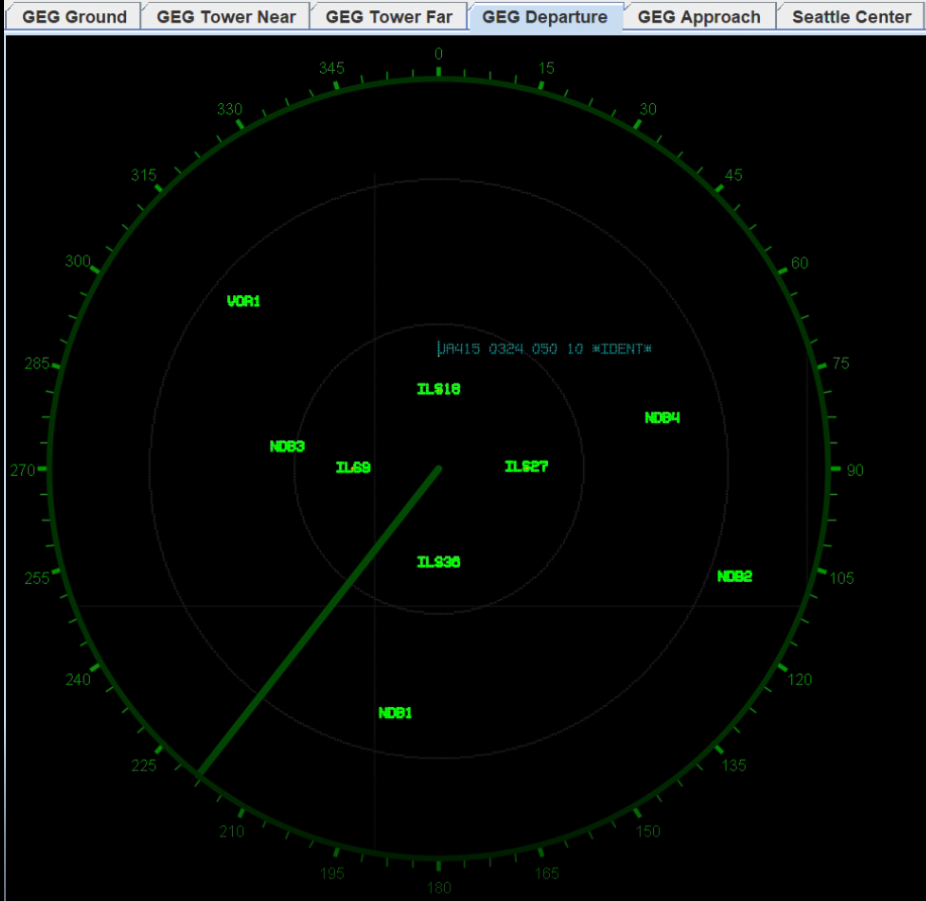
\includegraphics[scale=.23,valign=t,center]{test1.png}
\item The actual results are consistent with the expected results
\itemsep-.15cm
\item We could try changing an aircraft's transponder code to one that already exists and is being used by another aircraft to make sure that it doesn’t steal it away.
\end{enumerate}

\subsection{Test 2: Simple Straight Climb}
Instruct UA415 to climb straight ahead and maintain flight level 240.
\begin{enumerate}\itemsep-.15cm
\item This test verifies that an aircraft can climb to a new altitude and stop climbing and maintain its altitude once it reaches the target. This is mandatory for flying.
\item UA415 starts at an altitude of flight level 050 and is maintaining that altitude, and has a speed of 10
\item \begin{verbatim}UA415 climb and maintain flight level 240
\end{verbatim}
\item UA415 changes its altitude target to 240 and begins to climb. UA415 gradually climbs to 240 and then maintains that altitude once it reaches it. The speed and heading do not change.
\itemsep-.01cm
\item 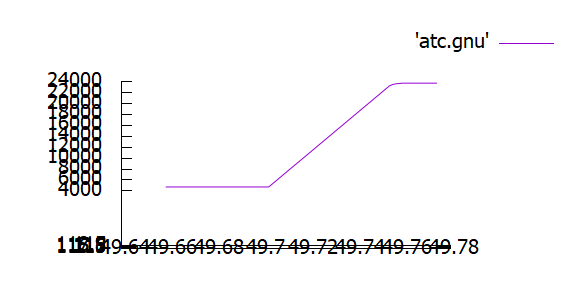
\includegraphics[scale=.55,valign=t,center]{test2.png}
\item The actual results are consistent with the expected results
\itemsep-.15cm
\item We could test descending to a different altitude to verify that decreasing altitude also works
\end{enumerate}

\subsection{Test 3: Compound Straight Climb}
Instruct UA415 to climb straight ahead and maintain flight level 320, then upon arriving descend to 15,000 feet.
\begin{enumerate}\itemsep-.15cm

\item This test verifies that the aircraft can increase in altitude and maintain it once it reaches its target, and then descend again shortly after. This is mandatory to depart and approach.
\item UA415 starts at an altitude of flight level 50 and is maintaining that altitude, and has a speed of 10
\item \begin{verbatim}UA415 climb and maintain flight level 320
UA415 descend and maintain 15000
\end{verbatim}
\item UA415 will start to climb to flight level 320. Once it reaches flight level 320 it will maintain it for a short amount of time. UA415 will then start to descend until it reaches 15,000 feet. It will then maintain that altitude. The speed stays the same throughout.
\itemsep-.01cm
\item 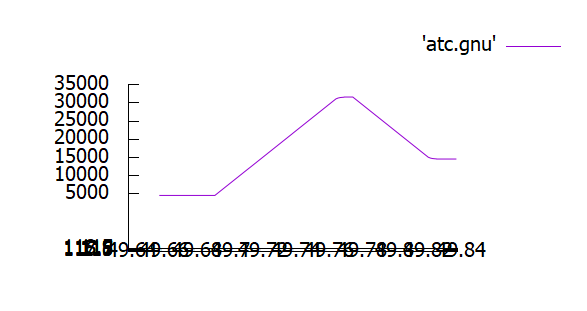
\includegraphics[scale=.55,valign=t,center]{test3.png}
\item The actual results are consistent with the expected results
\itemsep-.15cm
\item We could test descending past 0 feet to make sure that we won’t be able to make an aircraft do something life threatening.
\end{enumerate}

\subsection{Test 4: Simple Level Turn}
Instruct UA415 to turn right to 135 degrees.
\begin{enumerate}\itemsep-.15cm
\item This test verifies that an aircraft can perform a basic turn which is mandatory for every flight
\item UA415 starts and stays at a speed of 10. UA415 starts pointing at degree 0
\item \begin{verbatim}UA415 turn right to 135
\end{verbatim}
\item UA415 travels straight for some time then begins to turn right. UA415 stops turning once it is pointing in the direction of 135 degrees while staying at the same altitude and speed.
\itemsep-.01cm
\item 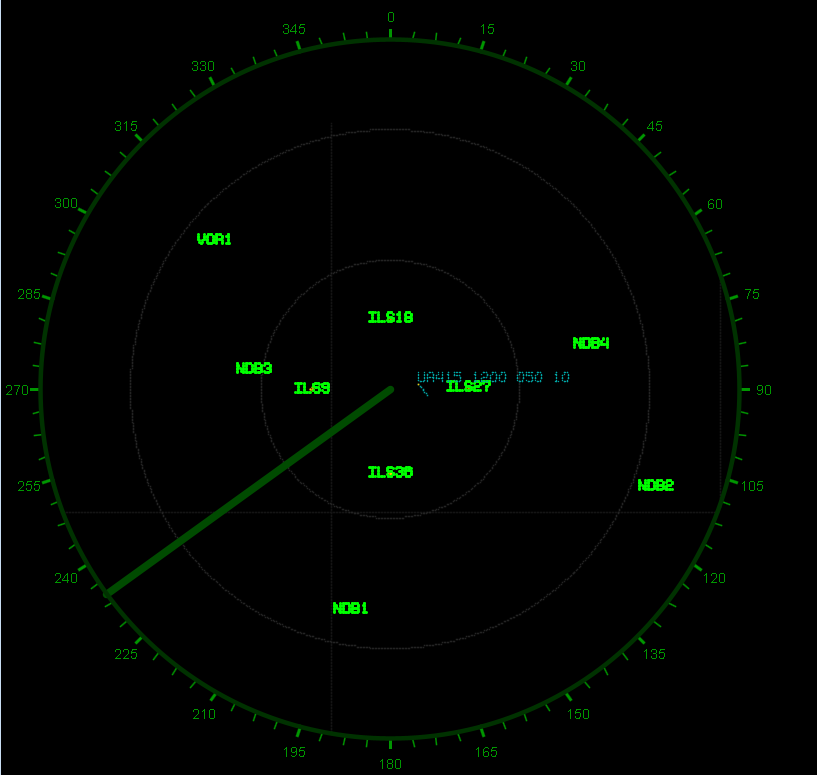
\includegraphics[scale=.25,valign=t,center]{test4_1.png}
\item The actual results are consistent with expected results
\itemsep-.15cm
\item We could test turning the aircraft left to 135 degrees to make sure it ends up pointing in the same direction.
\end{enumerate}

\subsection{Test 5: Compound Level Turn}
Instruct UA415 to turn left to 270 degrees, then upon arriving right to 090.
\begin{enumerate}\itemsep-.15cm
\item The test verifies that the aircraft can perform both right and left turns, one after the other. This is a mandatory maneuver for every flight
\item UA415 starts off at flight level 050 and points at 0 degrees. It is travelling at a speed of 10.
\item \begin{verbatim}UA415 turn left to 270
UA415 turn right to 090
\end{verbatim}
\item UA415 travels straight for some time. UA415 then turns left until it reaches 270 degrees. It then turns right until it reaches 90 degrees.
\itemsep-.01cm
\item 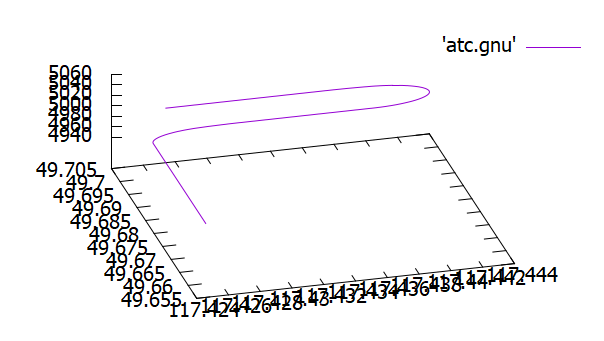
\includegraphics[scale=.55,valign=t,center]{test5.png}
\item The actual results are consistent with the expected results
\itemsep-.15cm
\item We could test doing a full 360 turn in both directions to make sure that it will actually turn
\end{enumerate}

\subsection{Test 6: Simple Speed Change}
Instruct UA415 to increase speed to 200 knots (entered as 20).
\begin{enumerate}\itemsep-.15cm
\item This test verifies that the \verb!increase speed! command correctly increases the speed of the aircraft so that the aircraft can change speed for basic maneuvering.
\item The aircraft UA415 starts flying North, then the speed is increased to 200 knots.
\item \verb!UA415 increase speed to 20!
\item The plane will change speed to the new increased speed and continue at the new speed of 200 knots until it arrives.
\itemsep-.01cm
\item 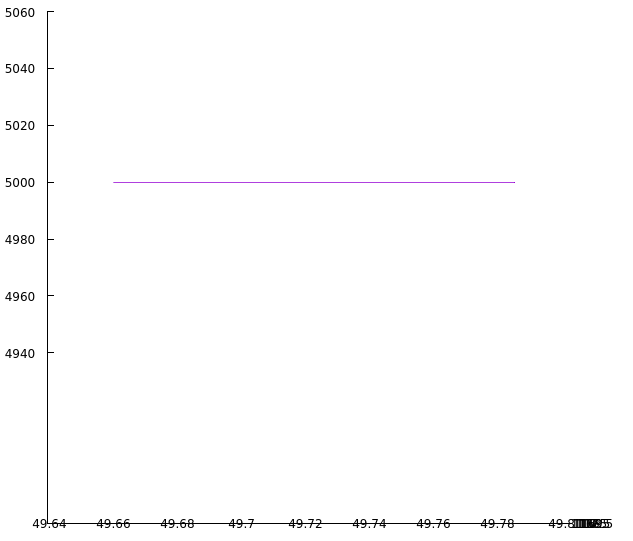
\includegraphics[scale=.45,valign=t,center]{test6.png}
\itemsep-.15cm
\item The actual results did not differ much from the expected results.
\item Test continual speed increase until a condition is met.
\end{enumerate}

\subsection{Test 7: Compound Speed Change}
Instruct UA415 to increase speed to 250 knots, then upon arriving reduce speed to 100.
\begin{enumerate}\itemsep-.15cm
\item This test verifies multiple speed changes can be executed and that \verb!reduce speed! can correctly reduce the speed of the aircraft for basic maneuvering.
\item The aircraft \verb!UA415! will start flying north traveling at a constant speed, then the speed will increase to 250 knots, then the speed will decrease to 100 knots.
\item \begin{verbatim}
UA415 increase speed to 25
UA415 reduce speed to 10
\end{verbatim}
\item The aircraft \verb!UA415! will travel at a constant speed of 250 knots, then as it approaches 250 knots, the speed will decrease to 100 knots traveling in the same direction.
\itemsep-.01cm
\item 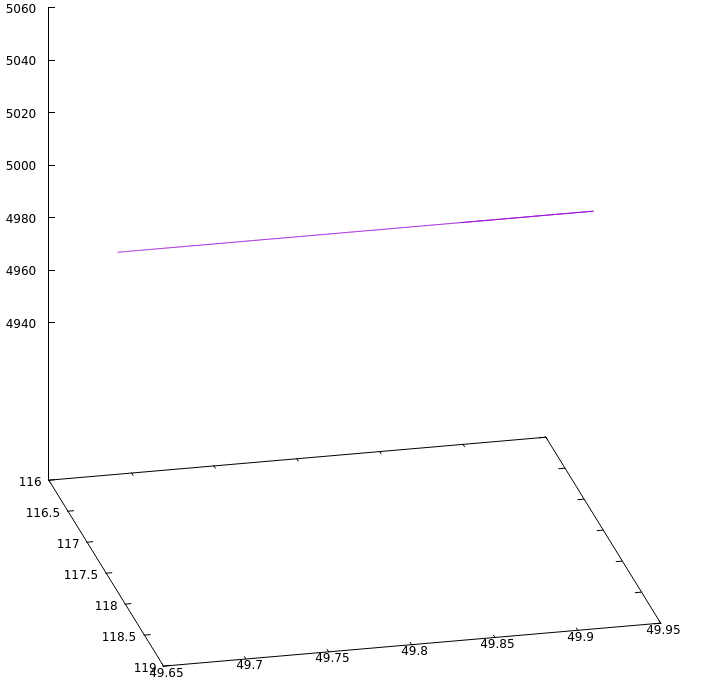
\includegraphics[scale=.4,valign=t,center]{test7.png}
\item The actual results drastically differ from expected results. The aircraft reversed direction upon the issuance of \verb!UA415 reduce speed to 10!.
\itemsep-.15cm
\item This test can be extended by adding a stop or wait.
\end{enumerate}

\subsection{Test 8: Descending Turn}
Instruct UA415 to climb to flight level 240 to start the test (ignore this setup in the results). Upon arriving, descend to 8,000 feet while turning left to 010.
\begin{enumerate}\itemsep-.15cm
\item This test verifies that the \verb!descend! and \verb!turn! commands will accurately direct the aircraft to descend into a left turn for basic navigation.
\item The aircraft \verb!UA415! will be flying north climbing at a constant speed to flight level 240. 
\item \begin{verbatim}
UA415 climb and maintain 240
UA415 turn left to 010
UA415 descend and mantain 8000
\end{verbatim}
\item The aircraft \verb!UA415! will climb at a constant speed to flight level 240, then as it approaches 240 flight level, \verb!UA415! will turn to 010 and descend to 8000.
\itemsep-.01cm
\item 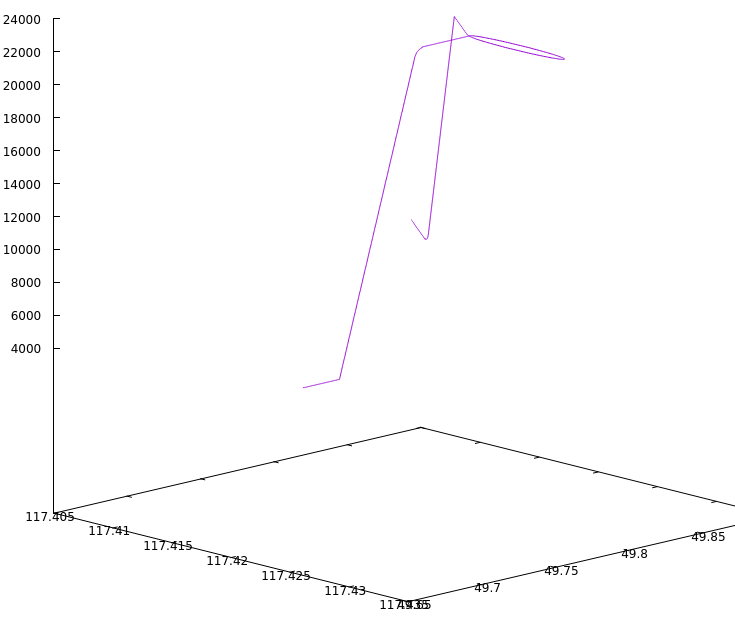
\includegraphics[scale=.4,valign=t,center]{test8.png}
\item The actual is generally expected, however the aircraft attempted to turn right as well.
\itemsep-.15cm
\item This test can be extended by adding another turn or descend or climb again in the case of avoiding obstacles.
\end{enumerate}

\subsection{Test 9: Turn Radius Comparison}
9a. Instruct UA415 to turn right to 270.\\
9b. Instruct UA415 to turn right to 270 and increase speed to 30.\\
9c. Instruct UA415 to turn right to 270 and increase speed to 50.
\begin{enumerate}\itemsep-.15cm
\item This test verifies turn accuracy when a turn radius is specified. We want to see correct behaviour when given a turn direction and radius as well a speed change to examine how the speed affects the turn radius. This is important for maneuvering the aircraft accurately and precisely.
\item A general English description of the conditions of the test.
\item \begin{enumerate}
    \item[9a.] \verb!UA415 turn right to 270!
    \item[9b.] \verb!UA415 turn right to 270!\\
        \verb!UA415 increase speed to 30!
    \item[9c.] \verb!UA415 turn right to 270!\\
        \verb!UA415 increase speed to 50!\\
    \end{enumerate}
\item The aircraft will turn to the right to 270. As the speed increases, the turn radius should increase.
\itemsep-.01cm
\item 9a. 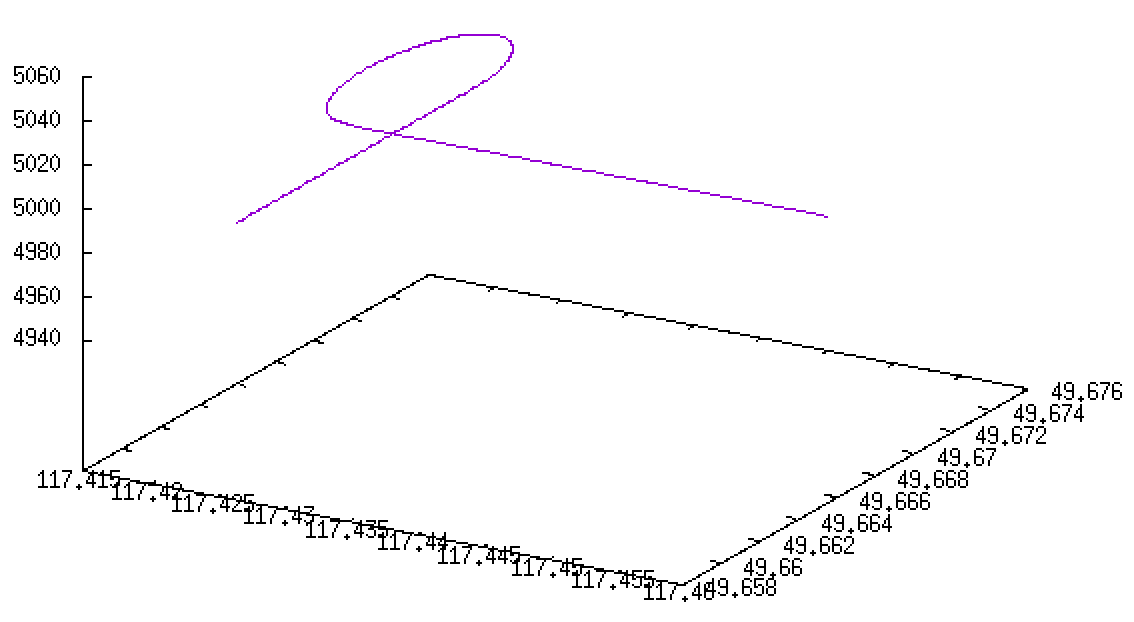
\includegraphics[scale=.35,valign=t]{test9_a.png} 9b.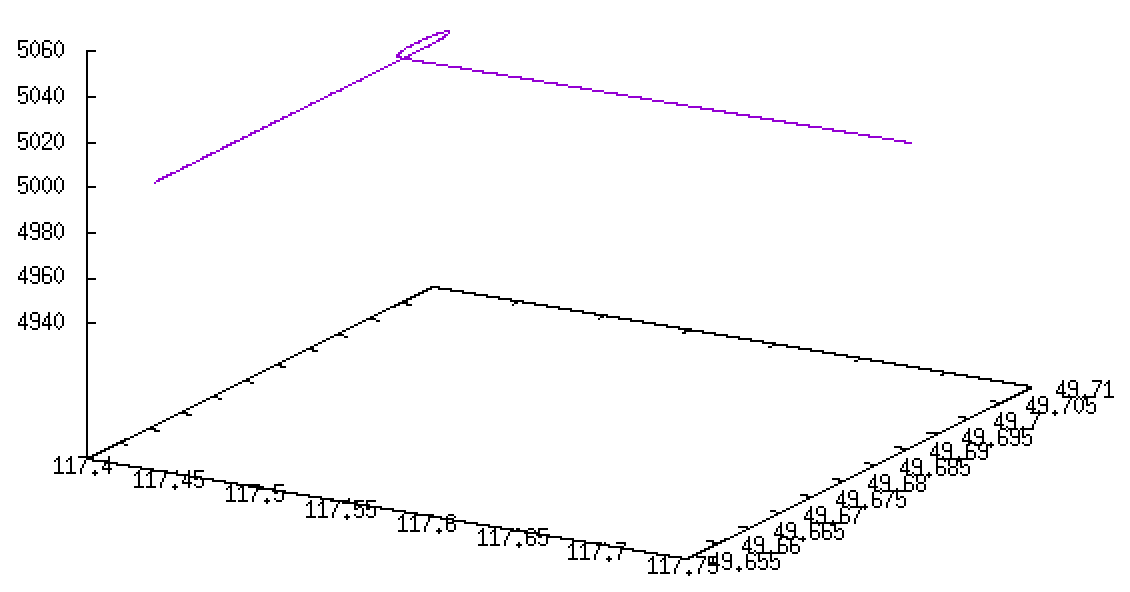
\includegraphics[scale=.35,valign=t]{test9_b.png}\\
9c. 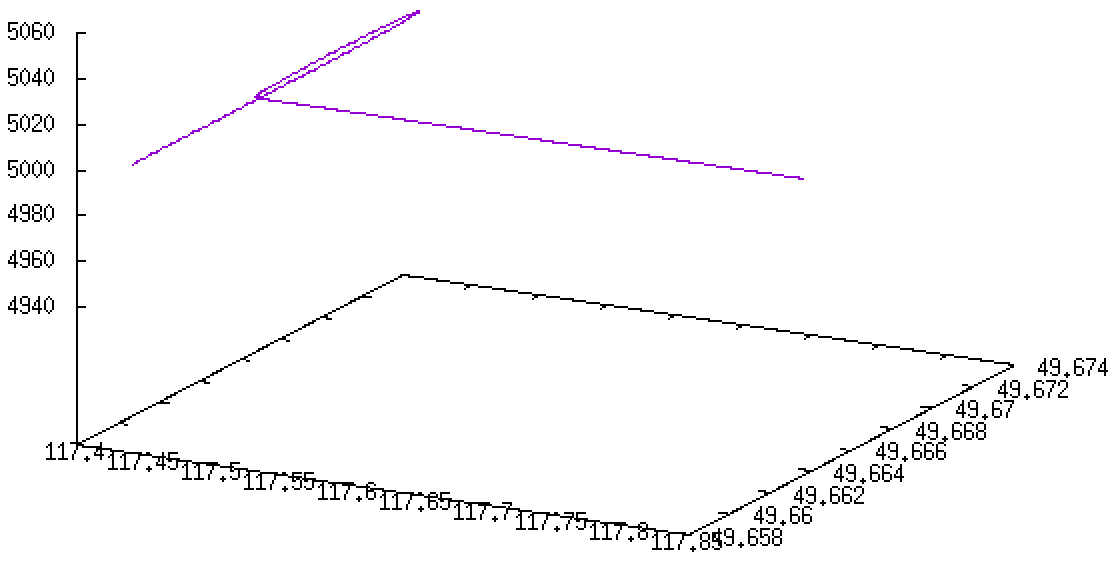
\includegraphics[scale=.35,valign=t]{test9_c.png}
\item The actual results are mostly as expected. The turn radius of test 9c, increasing the speed to 50, did increase the turn radius from the previous test that increased the speed to 30. The turn radius of the initial test is surprisingly larger than when the speed is increased to 30.
\itemsep-.15cm
\item This test can be extended by also comparing \verb!reduce speed!.
\end{enumerate}

\subsection{Test 10: Proceed to Fix, Level}
Instruct UA415 to proceed to fix NDB4.
\begin{enumerate}\itemsep-.15cm
\item This test verifies that the \verb!proceed! to fix command accurately directs the aircraft to the correct fix so the aircraft can follow controller instructions.
\item The aircraft will start flying north, then head toward NDB4.
\item \verb!UA415 proceed to ndb4!
\item The aircraft will navigate toward NDB4 upon issuance of the command.
\itemsep-.01cm
\item 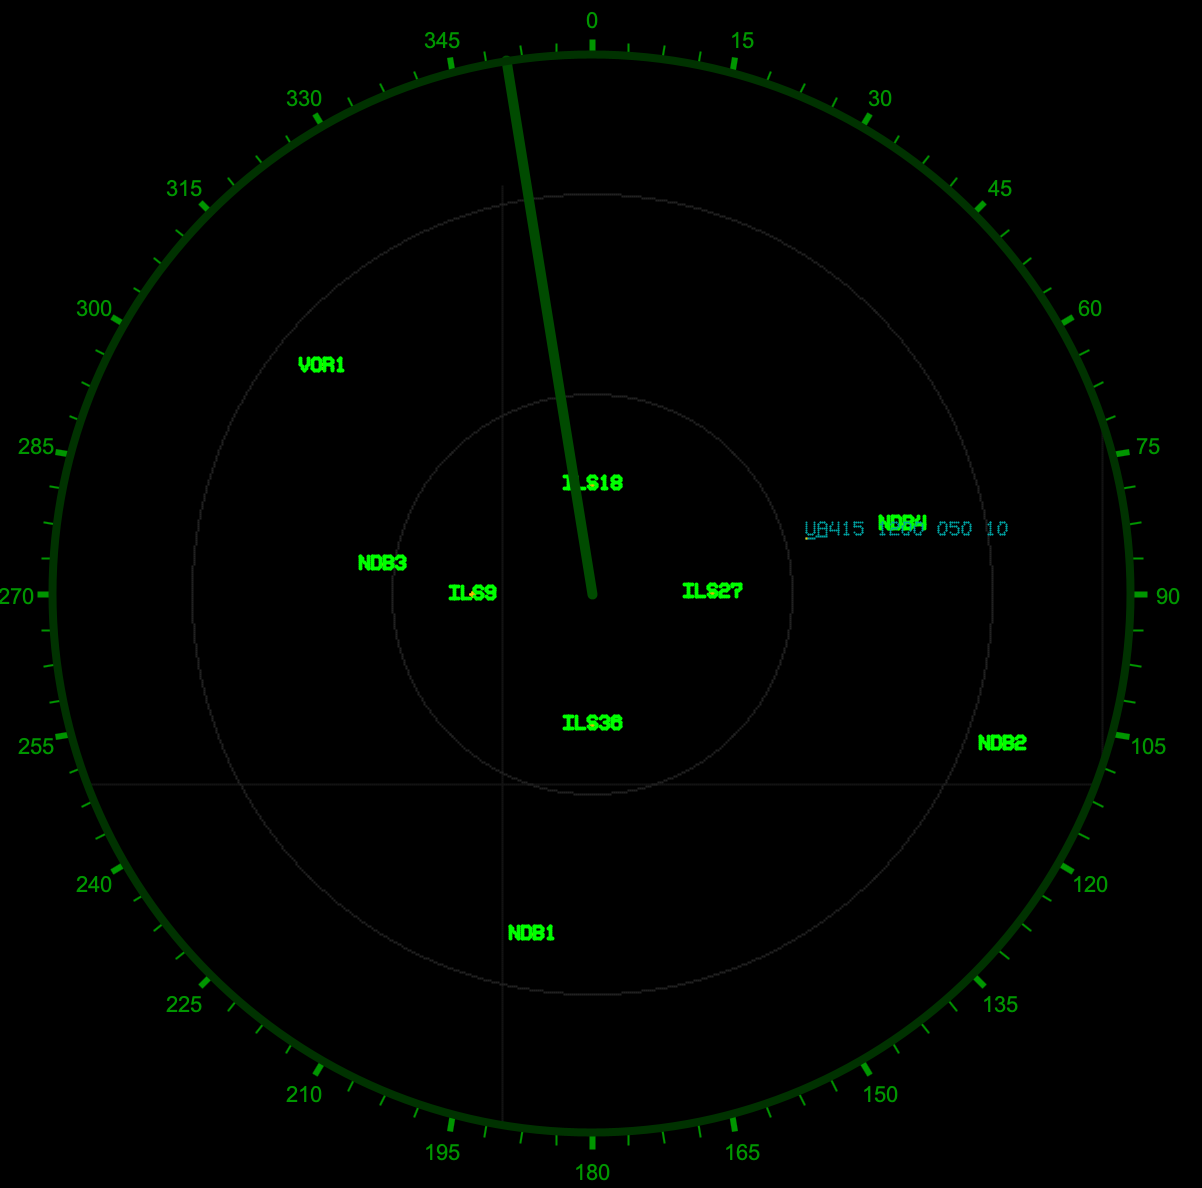
\includegraphics[scale=.3,valign=t]{test10_1.png}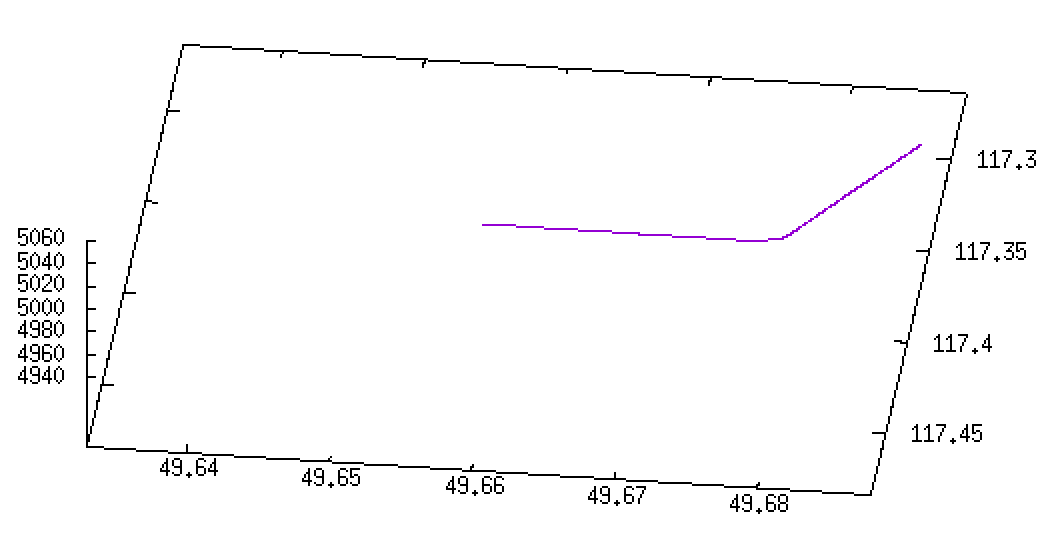
\includegraphics[scale=.5,valign=t]{test10_2.png}
\item The actual results are as expected.
\itemsep-.15cm
\item This test can be extended by adding another fix to the route.
\end{enumerate}

\subsection{Test 11: Proceed to Fix, Climbing}
Instruct UA415 to proceed to fix NDB4 and cross it at flight level 200.
\begin{enumerate}\itemsep-.15cm
\item It is testing the ability of the aircraft to navigate to NDB4 at an altitude of 200. The previous test just needed to see if the aircraft could head to the designated FIX, but now we care if it can do so while maintaining a specific flight level.
\item Pass over the location of NDB4 at flight level 200.
\item \verb!UA415 proceed to ndb4 cross at flight level 200!
\item We expect UA415 to pass over ndb4 at 200 flight level. It should turn and increase altitude to adjust.
\itemsep-.01cm
\item 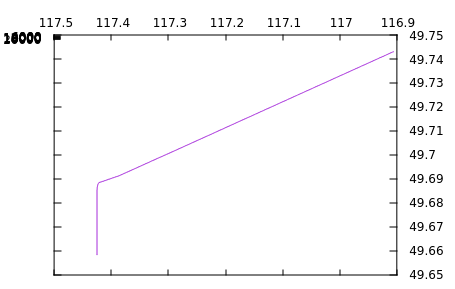
\includegraphics[scale=.6,valign=t]{test11_1.png} 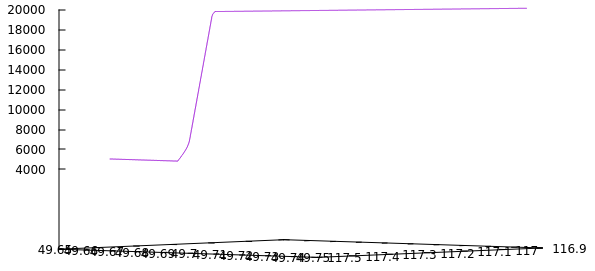
\includegraphics[scale=.5,valign=t]{test11_2.png}
\item The expected results match the actual results in this case.
\itemsep-.15cm
\item This test could be repeated for every fix. It can also be repeated for other flight levels (could create intervals of flight level tests, 100, 200, 50, etc).
\end{enumerate}

\subsection{Test 12: Proceed to Fixes, Altitude Changes}
Instruct UA415 to proceed to fix NDB4 and cross it at flight level 200, NDB2 at 100, NDB1 and 240.
\begin{enumerate}\itemsep-.15cm
\item This test is to see if UA415 can navigate between fixes at varying altitudes. It is common for aircraft to move from one fix to other fixes so this is an important ability for the simulator to be able to do.
\item Navigate to NDB4 at flight level 200, then navigate to NDB2 while dropping altitude to flight level 100, then turn and navigate to NDB1 while gaining altitude to flight level 240
\item \begin{lstlisting}
ua415 proceed to ndb4 cross at flight level 200 proceed to ndb2 proceed to ndb1
ua415 descend and maintain flight level 100
ua415 climb and maintain flight level 240
\end{lstlisting}
\item UA415 is expected to move to NDB4, then NDB2, then NDB1. It will climb to 200 initially. Input between NDB4 and NDB2 will descend its flight level to 100. Input between NDB2 and NDB1 will increase its flight level to 240.
\itemsep-.01cm
\item 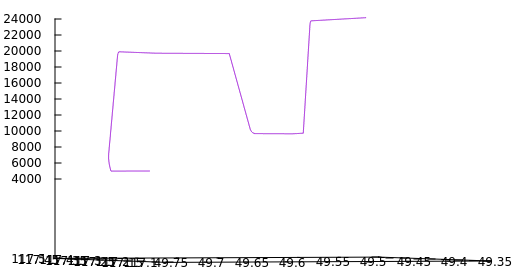
\includegraphics[scale=.6,valign=t]{test12_1.png} 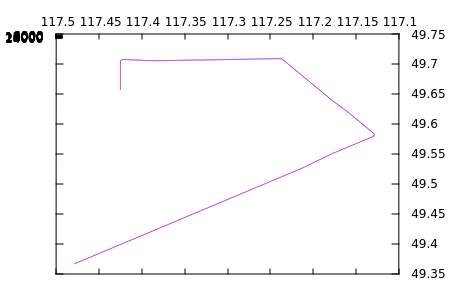
\includegraphics[scale=.6,valign=t]{test12_2.png}
\item The expected results matched the actual results.
\itemsep-.15cm
\item This test could be expanded on for the order of fix navigation (changing the order of NDB4, NDB2, NDB1). We could also add or subtract fixes involved in the test down to 2, and test each permutation of navigation. This would be extensive, but comprehensive.
\end{enumerate}

\subsection{Test 13: Proceed to Fix, Climbing and Hold 1}
Instruct UA415 to proceed to fix NDB3 and hold.
\begin{enumerate}\itemsep-.15cm
\item This test is to see if UA415 can maintain a holding procedure at a fix. There may be traffic or other conditions that require the aircraft to enter holding, so it is important to verify that the simulation can meet this requirement.
\item Navigate to NDB3, then enter the holding procedure.
\item \verb!ua415 proceed to ndb3 and hold!
\item Prediction is that UA415 will navigate to ndb3 then enter a holding procedure.
\itemsep-.01cm
\item 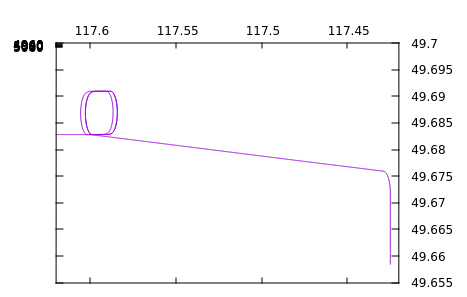
\includegraphics[scale=.6,valign=t]{test13_1.png} 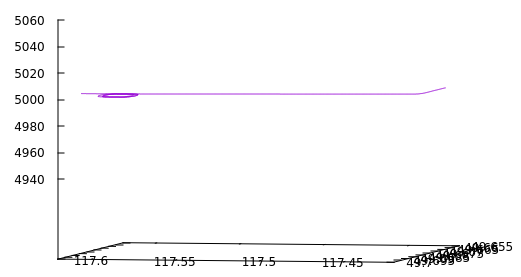
\includegraphics[scale=.57,valign=t]{test13_2.png}
\item The actual results differed from the expected as we predicted it entering holding, but not an estimate on how many passes or how long it would hold this position. It performed 3 ‘loops’, then left the position.
\itemsep-.15cm
\item This test could be extended to evaluate other fixes (as one other test does). We could also evaluate giving additional instructions after holding to see how that may affect what it does after holding.
\end{enumerate}

\subsection{Test 14: Proceed to Fix, Climbing and Hold 2}
Instruct UA415 to proceed to fix NDB4 and hold.
Explain how Tests 13 and 14 differ.
\begin{enumerate}\itemsep-.15cm
\item This test is to see if UA415 can maintain a holding procedure at a fix. There may be traffic or other conditions that require the aircraft to enter holding, so it is important to verify that the simulation can meet this requirement.
\item Navigate to NDB4, then enter the holding procedure.
\item \verb!ua415 proceed to ndb4 and hold!
\item The prediction is that this test will run an identical test as test 13. UA415 should navigate to NDB4, hold for 3 turns, then proceed in its prior direction of travel.
\itemsep-.01cm
\item 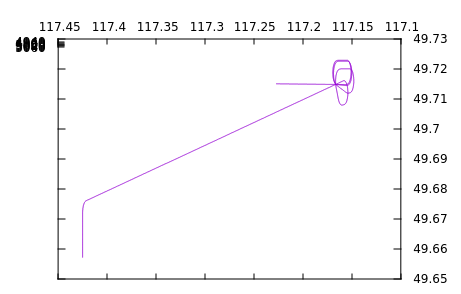
\includegraphics[scale=.6,valign=t,center]{test14_1.png}
\item Unlike how it was predicted, UA415 went West-bound after the holding position. It also made a loop maneuver to be able to enter the holding position. It looks like test 13 differs from test 14 in that the direction the aircraft is facing when it needs to enter the holding position changes how an aircraft enters holding position. The aircraft needs to be able to do holding in the same direction regardless of where it came from, so it would make sense that some adjustments need to be made.
\itemsep-.15cm
\item We can expand on this by observing how aircraft enter and leave holding when facing a more Northern or Southern heading.
\end{enumerate}

\subsection{Test 15: Proceed to Fix, Procedure Turn}
Instruct UA415 to proceed to fix NDB4 and execute the procedure turn for runway 22.
\begin{enumerate}\itemsep-.15cm
\item Instruct UA415 to navigate to NDB4 and do a procedure turn, aligning to runway 22. Properly aligning with the runway is an important step to landing on the runway.
\item Navigate to NDB4, then perform a procedure turn for a specific runway on NDB4.
\item \verb!ua415 cleared to ndb4 for procedure turn runway 22!
\item UA415 should navigate to NDB4. Once there, it should perform a procedure turn, ending in the direction of runway 22.
\itemsep-.01cm
\item In testing, UA415 proceeded to NDB4. It did a procedure turn once there and continued to go straight. Image below: procedure turn on the right hand of the screen shot, once arriving at NDB4

    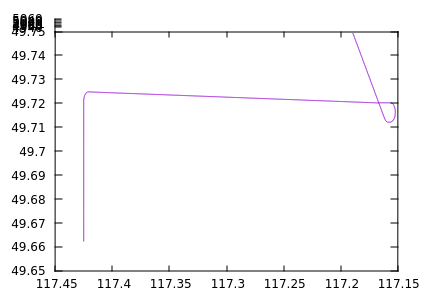
\includegraphics[scale=.6,valign=t,center]{test15_1.png}
\itemsep-.15cm
\item We were not sure the direction alignment of runway 22 at NDB4, so the final heading was unknown in our prediction. We also were unsure of the direction of the procedure turn. Other than the unknown quantities, the test performed as expected.
\item This test could be expanded on in many directions. We could perform procedure turns on every other fix in the test environment. We can also perform procedure turn for different runways at the fixes, as well as how the aircraft handles entering the procedure turn from holding, or how it would handle approaching procedure turn from different directions.
\end{enumerate}
\end{document}
